\documentclass[unnumsec,webpdf,contemporary,large]{oup-authoring-template}
\usepackage{hyperref}
\usepackage{xspace}
\usepackage{graphicx}
\newcommand{\zlib}{\texttt{zlib}\xspace}
\newcommand{\zran}{\texttt{zran}\xspace}
\newcommand{\ibuilder}{\texttt{index\_builder}\xspace}
\newcommand{\ireader}{\texttt{index\_reader}\xspace}
\newcommand{\gzip}{gzip\xspace}

\begin{document}

\journaltitle{CMSC701 Final Project}
\DOI{}
\copyrightyear{2023}
\pubyear{2023}
\appnotes{Final Project}

\firstpage{1}

%\subtitle{Subject Section}

\title[Compressed Checkpoint Index]{Final Project Report: Compressed Checkpoint
Index \& Parallel \gzip Reader}

\author[1]{Erik Rye}
\author[1]{Jiaxi Tang}
\author[1]{Aaron Ortwein}

%\authormark{Author Name et al.}

\address[1]{\orgdiv{Computer Science Department}, \orgname{University of
Maryland}, \orgaddress{\street{8125 Paint Branch Dr, College Park},
\postcode{20742}, \state{MD}, \country{USA}}}

%\corresp[$\ast$]{Corresponding author. \href{email:email-id.com}{email-id.com}}

%\received{Date}{0}{Year}
%\revised{Date}{0}{Year}
%\accepted{Date}{0}{Year}

\abstract{We devise and describe a tool for creating an index over a \gzip FASTQ
file. Unlike standard index-creation tools, our tool and the indices that it
creates incorporate a user-specified number of sequence reads that should be
split into each index. This allows a different tool that reads a FASTQ \gzip
file with our pre-built index over it to efficiently process the sequence reads
\emph{in parallel}, rather than needing to process the entire file serially.
This can result in a dramatic speedup for some applications, as we demonstrate
with the simple use case of reading the entire FASTQ file into memory and
writing the decompressed result back to a file.}

\keywords{FASTQ, \gzip, Compression, Parallel Processing}

% \boxedtext{
% \begin{itemize}
% \item Key boxed text here.
% \item Key boxed text here.
% \item Key boxed text here.
% \end{itemize}}

\maketitle


\section{Introduction}
Computer processors are now capable of running hundreds of threads of execution simultaneously in parallel. With severe physical limits on clock speed, future architectures will likely support more simultaneous threads rather than faster individual cores ~\cite{intropaper}. These advances provides programmers new way to speed up their programs. However, simply using more threads to exexute parts of the program does not guarantee speedup and may very well speed down than speed up. In fact, it is not uncommon for a program’s overall throughput to decrease when thread count grows large enough ~\cite{intropaper}. So, to speedup genomics software with multiple number of threads, programmers should deliberate on how they should structure the entire program and how many threads they should use so that the overhead of multithreading will not outweigh the speedup it brings.

Here we try to solve the problem of decompressing a gzip compressed FASTQ files in parallel by building indices over it. 
This startegies of building indices can scale to hundreds of threads and make it easier for our program to be part of the pipeline of other multithreading or multiprocessing genomics tools. 
\subsection{Challenge of Multithreading}
Some of the challenges multithreading will pose can be seen in Figure 1. Figure 1 shows how bad multithreading can be if handled incorrectly. We can see that if a thread needs to read from or write to a file, it needs exclusive right to the file so that the file won't be changed when it's reading it. This is usually done by using locks. Unfortunately, even though multiple threads can have read lock of the same file, operating system does not really allows them to read the file simultaneously. That means if multiple thread is trying to read a file, most of them cannot do anything and has to wait for that one thread to complete first. The same applies to writing to a file as well. Therefore, it's important to structure the program and choose parameters wisely so that the time spent waiting for each thread is minimum. 
\begin{figure}
    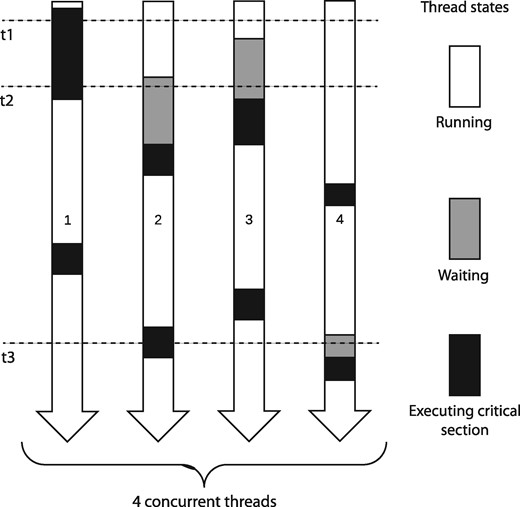
\includegraphics[width=\linewidth]{figs/multithread.jpeg}
    \label{fig:multithread}
    \caption{This figure shows 4 threads running simultaneously . Time progress from top to bottom. Gray area represents time spent waiting instead of operating. Black area represents threads doing operations that require exclusive rights to certain resources. ~\cite{intropaper}}
\end{figure}

\section{Related Work}

Kerbiriou and Chikhi examined parallel decompression of FASTQ \gzip files to
speed up genomic algorithms that require FASTQ
input~\cite{kerbiriou2019parallel}. They do not build an index over the FASTQ
file by making a pass over it as we attempt to do, but rather attempt to
reconstruct data from back-references discovered by reading forward from a
random entry point.

\texttt{zlib}~\cite{zlib} is a C library written by Mark Adler and others that
is able to create and read \gzip files. This library will be important for our
project as it exposes the underlying mechanics for inflating \gzip files.

\texttt{pyfastx}~\cite{pyfastx} is a Python C extension that enables random
reads from FASTA and FASTQ. The functionality that it exposes is similar to our
overall goal and will be a useful source of information and point of comparison.

\texttt{indexed\_gzip}~\cite{indexedgzip} is a project by Paul McCarthy to
create an index over compressed NIFTI image files, which use \gzip compression by
default. This will be another useful point of comparison in a tool that needs to
accomplish a similar task as us.

\begin{table*}[ht]
    \centering
    \caption{Four sources of FASTQ data were used in our study. The FASTQ files
    were \gzip compressed for our index-building and parallel reading
    experiments.}
\begin{tabular}{r|l|r|r}
\multicolumn{1}{c}{\textbf{\begin{tabular}[c]{@{}c@{}}Sequence Read\\
Identifier\end{tabular}}} & \multicolumn{1}{c}{\textbf{Source}} &
    \multicolumn{1}{c}{\textbf{Sequence Reads}} & \multicolumn{1}{c}{\textbf{\begin{tabular}[c]{@{}c@{}}FASTQ GZ \\ Size (MB)\end{tabular}}} \\
\hline\\
SRR3295681 (Small)& Salmonella enterica & 959,879 & 205\\
SRR2121685 (Medium) & Mus musculus & 27,928,438 & 2,078\\
SRR925811  (Large) & Homo sapiens & 53,265,409 & 3,349 \\
SRR925816 (XL) & Homo sapiens & 71,504,007 & 5,046
\end{tabular}
    \label{tab:source}
\end{table*}

\section{Methodology}

The software tools we developed for our project consist of an \emph{index
building} component, which creates the sequence-aware \gzip index, and an
\emph{index reading} component, which we use to validate the utility of the
index building component by using the indices to read a compressed gzip file in
parallel and write it out to a file, which we then compare against the
uncompressed original FASTQ to verify our program's correctness. We first detail
the thought process and inspriation behind our approach in
Section~\ref{sec:zran}, document the design of our index builder in
Section~\ref{sec:ibuilder}, and discuss the design of the index reader and validation
tool in Section~\ref{sec:ireader}.

\subsection{\zran}
\label{sec:zran}

The starting point for our index creation utility is a tool called
\zran~\cite{zran}. \zran
is a single-file demonstration of how to build an index over a \gzip file
written by Mark Adler, co-creator and maintainer of \zlib. It is included with
\zlib. \zran is designed to allow for random access within a \gzip file. \zran
accomplishes this in two steps. First, we describe the low-level internals of
how \zlib accomplishes compression and decompression, then we describe each of
the steps in \zran.

First, \zran completes a full read through the \gzip file. At each \gzip block
boundary (which which is anno)

\subsection{\ibuilder}
\label{sec:ibuilder}

\subsection{\ireader}
\label{sec:ireader}

\subsection{Data Sources}

We used four reference FASTQ sequence reads from the Sequence Read
Archive~\cite{SRA} for our testing and analysis. Table~\ref{tab:source} is a
tabular depiction of the data sets that we used for this project. We chose these
files because they represented a wide range of numbers of sequence reads, which
translates into a wide range of \gzip file sizes for our tool to contend with.
Indeed, the largest FASTQ \gzip file we consider is approximately 25 times as
large as the shortest.

\subsection{Index Creation Tool \& Methodology}

We implemented our solution in C in order to take advantage of the library
\zlib~\cite{zlib}. \zlib is a C library written and maintained by Jean-loup
Gailly and Mark Adler since 1995. 

\subsection{Parallel Reading}


\begin{figure}
    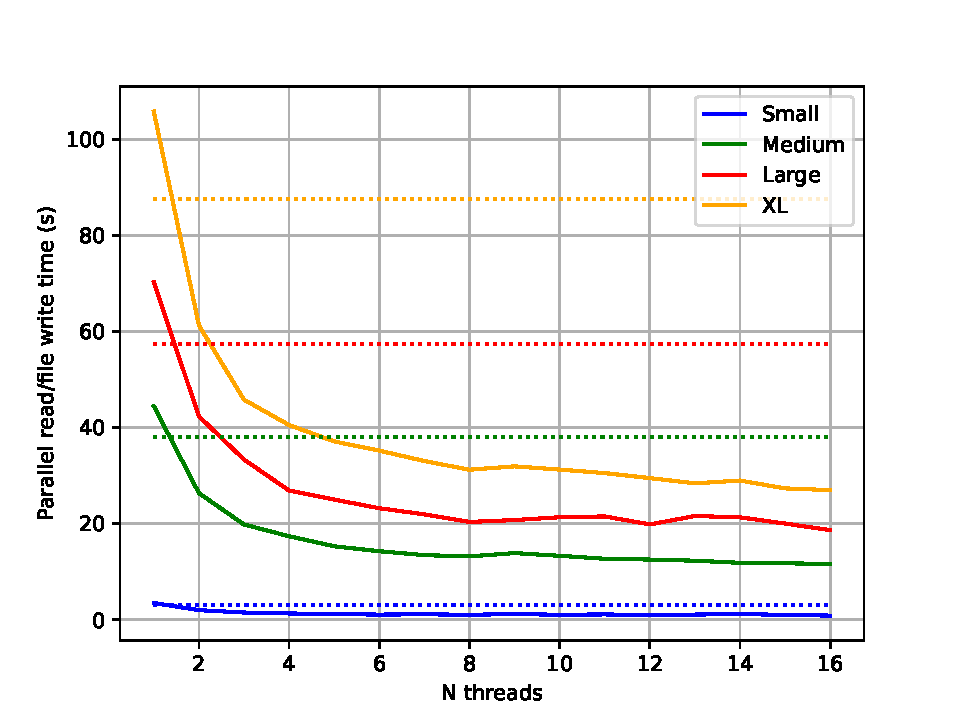
\includegraphics[width=\linewidth]{figs/cores.pdf}
    \label{fig:cores}
    \caption{Time to read differently-sized FASTQ \gzip files using a pre-built
    index file and different numbers of threads. Time compasses total program
    execution, including reading the index files, parallel reading the \gzip
    file with $N$ threads, and writing the reconstituted file to disk. Time for
    \texttt{zcat} to read the file and write it to disk is shown for comparison
    using a dotted line (\texttt{zcat} execution is single threaded). See
    Table~\ref{tab:source} for descriptions of small, medium, large, and XL.}
\end{figure}


\section{Results}

\section{Conclusion and Future Work}

Our work is located here:
\url{https://github.com/Josh-Tang112/CMSC701_Final_Project}

\bibliographystyle{plain}
\bibliography{refs.bib}


\end{document}
